% Example file for 60th International Conference paper
\documentclass{aes60i}
\usepackage{etex}
\usepackage{epsfig}
\usepackage{amsmath}
\usepackage{multirow}
\usepackage{tabularx}
\usepackage{booktabs}
\usepackage{amsmath,graphicx}
\usepackage{pgf}
\usepackage{tikz}
\usepackage{subfig}
\usetikzlibrary{backgrounds,shapes,snakes}
\usetikzlibrary{calc,chains,positioning}
\usepackage{phaistos}
\usepackage{cases}
\usepackage{pgfplots}
%\usepackage{empheq}
\usepackage{cite}

\hyphenation{Post-Script}

 
\authors{Ina Kodrasi and Simon Doclo\thanks{This work was supported in part by a Grant from the GIF, the German-Israeli Foundation for Scientific
    Research and Development, the Cluster of Excellence 1077 ``Hearing4All'', funded by the German Research Foundation (DFG), and the Marie Curie Initial Training Network DREAMS (Grant no. 316969).}}

\affiliation{University of Oldenburg, Dept. of Medical Physics and Acoustics, and Cluster of Excellence Hearing4All, Oldenburg, Germany}

\correspondence{Ina Kodrasi}{ina.kodrasi@uni-oldenburg.de}

\lastnames{Kodrasi, Doclo}

\title{INCORPORATING THE NOISE STATISTICS IN ACOUSTIC MULTI-CHANNEL EQUALIZATION}

\shorttitle{Incorporating the noise statistics in equalization}


\begin{abstract}
Acoustic multi-channel equalization techniques, such as the regularized partial multi-channel equalization technique based on the multiple-input/output inverse theorem (RP-MINT), are able to achieve a high dereverberation performance in the presence of room impulse response perturbations but may lead to additive noise amplification.
This paper proposes to directly extend the RP-MINT technique by incorporating the noise statistics in the reshaping filter design, such that joint dereverberation and noise reduction is achieved.
In addition to the regularization parameter used in the RP-MINT technique, a weighting parameter is introduced to trade off between dereverberation and noise reduction.
To automatically determine the regularization and weighting parameters, a novel non-intrusive procedure based on the L-hypersurface is proposed.
Simulation results using instrumental performance measures show that the proposed technique maintains the high dereverberation performance of the RP-MINT technique, while improving the noise reduction performance.
\end{abstract}

\begin{document}
\newlength\figureheight
\newlength\figurewidth
\setlength\figureheight{2.5cm}
\setlength\figurewidth{0.5\textwidth}

\maketitle 


\section{Introduction}

Speech signals recorded in an enclosed space by microphones placed at a distance from the source are often corrupted by reverberation and additive noise, which typically degrade speech quality, impair speech intelligibility, and decrease the performance of automatic speech recognition systems~\cite{Beutelmann_2006,Sehr_phd,Maas_ICASSP_2012}. 
With the continuously growing demand for high-quality hands-free speech communication, speech enhancement techniques aiming at joint dereverberation and noise reduction have become indispensable.
In this paper, we focus on the effective integration of the dereverberation and noise reduction tasks using acoustic multi-channel equalization techniques.
\newline
Acoustic multi-channel equalization techniques~\cite{Miyoshi_ITASS_1988,Kallinger_ICASSP_2006,Zhang_IWAENC_2010,Kodrasi_ITASLP_2013,Lim_ITASLP_2014} aim to reshape the measured or estimated room impulse responses~(RIRs) between the speech source and the microphone array. 
These techniques comprise in principle an attractive approach to speech dereverberation since in theory perfect dereverberation can be achieved~\cite{Miyoshi_ITASS_1988}.
In practice however, such techniques suffer from several drawbacks. 
Since the available (measured or estimated) RIRs typically differ from the true RIRs due to fluctuations (e.g., temperature or position variations~\cite{Radlovic_ITSA_2000}) or due to the sensitivity of supervised and blind system identification methods to near-common zeros and interfering noise~\cite{Haque_SPL_2008,Lin_ITASLP_2012}, such techniques can fail to achieve dereverberation and possibly cause additional speech distortion in the output signal~\cite{Zhang_IWAENC_2010,Kodrasi_ITASLP_2013}.
Furthermore, acoustic multi-channel equalization techniques typically design reshaping filters aiming only at speech dereverberation, without taking the presence of the additive noise into account. 
Applying such dereverberation filters may result in a large noise amplification~\cite{Kodrasi_ITASLP_2013}.
\newline
To increase the robustness against RIR perturbations, several techniques have been proposed~\cite{Zhang_IWAENC_2010,Kodrasi_ITASLP_2013,Lim_ITASLP_2014}, with the regularized partial multi-channel equalization technique based on the multiple-input/output inverse theorem~(RP-MINT) shown to yield a high dereverberation performance~\cite{Kodrasi_ITASLP_2013}.
By incorporating regularization in the RP-MINT technique, the energy of the reshaping filter is decreased, reducing the distortions in the output signal due to RIR perturbations, and hence, increasing the dereverberation performance. 
While the regularization parameter introduced in the RP-MINT technique is also effective in partly avoiding the additive noise amplification, the noise reduction performance is limited since the actual noise statistics are not explicitly taken into account.
\newline
In this paper we propose to directly extend the RP-MINT technique by explicitly taking the actual noise statistics into account such that joint dereverberation and noise reduction is achieved. 
In addition to the regularization parameter used in the RP-MINT technique, a weighting parameter is introduced, which enables to trade off between dereverberation and noise reduction.
Furthermore, a novel procedure for the joint automatic selection of the regularization and weighting parameters is also proposed.
Simulation results show that the proposed technique maintains the high dereverberation performance of the RP-MINT technique, while improving the noise reduction performance.\footnote{An extensive theoretical and experimental analysis of the technique proposed here is provided in~\cite{Kodrasi_ITASLP_2015}.}

\section{Configuration and Notation}

Consider the acoustic system depicted in Fig.~\ref{fig: configuration}, consisting of a single speech source, $M$ microphones, and additive noise.
Each microphone signal $y_m(n)$, $m = 1, \; \ldots, \; M$, at discrete-time index $n$, consists of a filtered version of the clean speech signal $s(n)$ and a noise component $v_m(n)$, i.e., 
\begin{equation}
\label{eq: tds1}
y_m(n)  = h_m(n) \ast s(n) + v_m(n) = x_m(n) + v_m(n),
\end{equation}
where $h_m(n)$ is the RIR between the speech source and the $m$-th microphone, $x_m(n)$ is the reverberant speech component at the $m$-th microphone, and $\ast$ denotes convolution.
Since the RIR $h_m(n)$ consists of a direct path and early reflections component $h_{e,m}(n)$ and a late reflections component $h_{r,m}(n)$, i.e., $h_{m}(n) = h_{e,m}(n) + h_{r,m}(n)$, the microphone signal in~(\ref{eq: tds1}) can also be written as
\begin{equation}
\label{eq: ysp}
y_m(n)  = \underbrace{h_{e,m}(n) \ast s(n)}_{x_{e,m}(n)} + \underbrace{h_{r,m}(n) \ast s(n)}_{x_{r,m}(n)} + \; v_m(n),
\end{equation}
with $x_{e,m}(n)$ the early reverberation component and $x_{r,m}(n)$ the late reverberation component at the $m$-th microphone.
Using the filter-and-sum structure in Fig.~\ref{fig: configuration}, the enhanced output signal $z(n)$ is equal to the sum of the filtered microphone signals, i.e., 
\begin{figure}[b!]
\centering
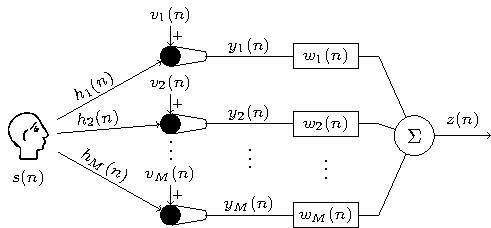
\includegraphics[scale=0.8]{Plots/configuration.pdf}
\caption{Schematic illustration of a typical time-domain multi-channel speech enhancement system.}
\label{fig: configuration}
\end{figure}
\begin{equation}
\label{eq: outcomp}
z(n) = \underbrace{\sum_{m=1}^M x_m(n) \ast w_m(n)}_{z_x(n)}  + \underbrace{\sum_{m=1}^M v_m(n) \ast w_m(n)}_{z_v(n)},
\end{equation}
where $w_m(n)$ is the filter applied to the $m$-th microphone, $z_x(n)$ is the output speech component, and $z_v(n)$ is the output noise component.
The output speech component can also be written as
\begin{equation}
z_x(n) = s(n) \ast \underbrace{\sum_{m = 1}^M h_m(n) \ast w_m(n)}_{c(n)},
\end{equation}
with $c(n)$ the equalized impulse response~(EIR) between the clean speech signal $s(n)$ and the output speech component $z_x(n)$.
Furthermore, the early reverberation output speech component $z_{e,x}(n)$ and the late reverberation output speech component $z_{r,x}(n)$ are defined as
\begin{align}
\label{eq: er_out}
z_{e,x}(n) & = \sum_{m=1}^M x_{e,m}(n) \ast w_m(n), \\
\label{eq: rr_out}
z_{r,x}(n) & = \sum_{m=1}^M x_{r,m}(n) \ast w_m(n).
\end{align}
In vector notation, the RIR $\mathbf{h}_m$ and the filter $\mathbf{w}_m$ are given by
\begin{align}
\mathbf{h}_m &= [h_m(0) \; h_m(1) \; \ldots \; h_m(L_h-1)]^T, \\
\mathbf{w}_m &= [w_m(0) \; w_m(1) \; \ldots \; w_m(L_h-1)]^T,
\end{align}
with $L_h$ and $L_w$ the RIR and the filter length respectively.
Using the $ML_w$-dimensional stacked filter vector $\mathbf{w}$, i.e., $\mathbf{w} = [\mathbf{w}^T_1 \; \mathbf{w}^T_2 \; \ldots \; \mathbf{w}^T_M]^T$, the EIR vector $\mathbf{c}$ of length $L_c$, i.e., $\mathbf{c} = [c(0) \; c(1) \; \ldots \; c(L_c-1)]^T$, is equal to
\begin{equation}
\label{eq: eir}
\mathbf{c} = \mathbf{H}\mathbf{w},
\end{equation}
with $\mathbf{H}$  the $L_c \times ML_w$-dimensional multi-channel convolution matrix.
Using the $ML_w$-dimensional stacked vector of the received microphone signals
\begin{equation}
\mathbf{y}(n) = \mathbf{x}(n) + \mathbf{v}(n),
\end{equation}
with
\begin{align}
\label{eq: ymn}
\mathbf{y}(n) & = [\mathbf{y}^T_1(n) \; \mathbf{y}^T_2(n) \; \ldots \; \mathbf{y}^T_M(n)]^T, \\
\mathbf{y}_m(n) & = [y_m(n) \; y_m(n-1) \; \ldots \; y_m(n-L_w+1)]^T,
\end{align}
and $\mathbf{x}(n)$ and $\mathbf{v}(n)$ similarly defined, the enhanced output signal $z(n)$ can be expressed as
\begin{equation}
z(n) =  \mathbf{w}^T\mathbf{x}(n) + \mathbf{w}^T\mathbf{v}(n) = \underbrace{\mathbf{w}^T\mathbf{H}^T}_{\mathbf{c}^T}\mathbf{s}(n) + \mathbf{w}^T\mathbf{v}(n),
\end{equation}
with $\mathbf{s}(n) = [s(n) \; s(n-1) \; \ldots \; s(n-L_c-1)]^T$ and $\mathbf{x}(n) = \mathbf{H}^T \mathbf{s}(n)$.
For conciseness, the time index $n$ will be omitted when possible in the remainder of this paper.

\section{Acoustic Multi-Channel Equalization Techniques}
\label{sec: ame}

Acoustic multi-channel equalization techniques typically disregard the presence of the additive noise $\mathbf{v}$ and design the reshaping filter $\mathbf{w}$ such that only the EIR $\mathbf{c}$ is optimized. 
Since the presence of the additive noise is disregarded, such techniques can result in a large noise amplification~\cite{Kodrasi_ITASLP_2013}~(cf. Section~\ref{sec: exp}).
Furthermore, since in practice only the perturbed RIRs $\hat{h}_m$ are available, the perturbed convolution matrix $\hat{\mathbf{H}} = \mathbf{H} + \mathbf{E}$ is used for the reshaping filter design, with $\mathbf{E}$ the convolution matrix of the RIR perturbations.
\newline
In this paper we will focus on the partial multi-channel equalization technique based on the multiple-input/output inverse theorem~(P-MINT) proposed in~\cite{Kodrasi_ITASLP_2013}, which aims at suppressing the late reverberation and preserving the perceptual speech quality. 
To this purpose, the late reflection taps of the target EIR $\mathbf{c}_t$ are set equal to $\mathbf{0}$, while the remaining taps are set equal to the direct path and early reflections of one of the available RIRs, i.e., 
\begin{equation}
\mathbf{c}_t = [\; \underbrace{\hat{h}_p(0) \; \ldots \; \hat{h}_p(L_d-1)}_{L_d} \; 0 \; \ldots \; 0 \; ]^{T},
\end{equation}
where $L_d$ corresponds to the length of the direct path and early reflections and $p \in \{1, \; 2, \; \ldots, \; M \}$.
The P-MINT filter is computed by minimizing the least-squares cost function
\begin{equation}
\label{eq: cost_p}
J_{_{\text{P}}} = \|\hat{\mathbf{H}}\mathbf{w} - \mathbf{c}_t \|_2^2.
\end{equation}
As shown in~\cite{Miyoshi_ITASS_1988}, assuming that the available RIRs do not share any common zeros and using $L_w \geq \left\lceil{\frac{L_h-1}{M-1}}\right\rceil$, the P-MINT filter minimizing the least-squares cost function in~(\ref{eq: cost_p}) is equal to
\begin{equation}
\label{eq: w_pmint}
\mathbf{w}_{_{\text{P}}} = \hat{\mathbf{H}}^+\mathbf{c}_t,
\end{equation}
where $\{ \cdot \}^+$ denotes the matrix pseudo-inverse. 
% Since the estimated convolution matrix is assumed to be a full row-rank matrix~\cite{Harikumar_ITSP_1998}, its pseudo-inverse can be computed as $\hat{\mathbf{H}}^+ = \hat{\mathbf{H}}^T(\hat{\mathbf{H}}\hat{\mathbf{H}}^T)^{-1}$.
When the true RIRs are available, i.e., $\hat{\mathbf{H}} = \mathbf{H}$, the P-MINT filter yields perfect dereverberation performance, i.e., $\mathbf{H}\mathbf{w}_{_{\text{P}}} = \mathbf{c}_t$.
However, in the presence of RIR perturbations, i.e., $\hat{\mathbf{H}} \neq \mathbf{H}$, applying the P-MINT filter to the true convolution matrix yields
\begin{equation}
\label{eq: lsout}
\mathbf{H}\mathbf{w}_{_{\text{P}}} = \hat{\mathbf{H}} \mathbf{w}_{_{\text{P}}} - \mathbf{E}\mathbf{w}_{_{\text{P}}} = \mathbf{c}_t - \mathbf{E}\mathbf{w}_{_{\text{P}}}.
\end{equation}
The first term in~(\ref{eq: lsout}) is the target EIR, whereas the second term represents distortions due to RIR perturbations.
If the energy of the reshaping filter $\mathbf{w}$ is small, then the distortions caused by RIR perturbations are also small.
To decrease the reshaping filter energy, and hence, to increase the robustness of the P-MINT technique against RIR perturbations, the RP-MINT technique has been proposed in~\cite{Hikichi_EURASIP_2007,Kodrasi_ITASLP_2013}.
The RP-MINT cost function is given by
% As shown in~\cite{Hikichi_EURASIP_2007}, when taking the RIR perturbations into account, an optimal reshaping filter in the minimum mean-square error sense can be computed by minimizing the cost function
% \begin{equation}
% \label{eq: c_E}
% J = \| \hat{\mathbf{H}}\mathbf{w} - \mathbf{c}_t\|_2^2 + \mathbf{w}^T {\cal{E}}\{\mathbf{E}^T\mathbf{E} \}\mathbf{w},
% \end{equation}
% where it is assumed that ${\cal{E}}\{\mathbf{E} \} = \mathbf{0}$.
% The matrix ${\cal{E}}\{\mathbf{E}^T\mathbf{E} \}$ in~(\ref{eq: c_E}) obviously depends on the energy and the type of RIR perturbations, e.g., perturbations arising due to microphone position fluctuations~\cite{Radlovic_ITSA_2000,Jungmann_ITASLP_2012}, or perturbations arising from blind or supervised system identification methods~\cite{Haque_SPL_2008,Lin_ITASLP_2012,Lim_IWAENC_2014}.
% While statistical models have been developed for the correlation structure of different types of perturbations, the exact ${\cal{E}}\{\mathbf{E}^T \mathbf{E} \}$ cannot be known in practice. 
% To account for inaccuracies in modeling ${\cal{E}}\{\mathbf{E}^T\mathbf{E} \}$, regularized acoustic multi-channel equalization techniques introduce a regularization parameter $\delta$ and use ${\cal{E}}\{ \mathbf{E}^T \mathbf{E} \} = \delta \mathbf{R}_{e}$, with $\mathbf{R}_{e}$ constructed based on a perturbation model~\cite{Jungmann_ITASLP_2012, Lim_IWAENC_2014}. 
% When no knowledge about the perturbations is available, they are often assumed to be spatially and temporally white, i.e., ${\cal{E}}\{\mathbf{E}^T \mathbf{E} \} = \delta \mathbf{I}$, with $\mathbf{I}$ denoting the $ML_w \times ML_w$-dimensional identity matrix~\cite{Hikichi_EURASIP_2007,Kodrasi_ITASLP_2013}.
% Using ${\cal{E}}\{ \mathbf{E}^T \mathbf{E} \} = \delta \mathbf{R}_{e}$ in~(\ref{eq: c_E}), the RP-MINT cost function is given by~\cite{Kodrasi_ITASLP_2013}
\begin{equation}
  \label{eq: rlscost}
  J_{_{\text{RP}}} =  \underbrace{\| \hat{\mathbf{H}}\mathbf{w} - \mathbf{c}_t \|_2^2}_{\epsilon_{{c}}} + \delta \underbrace{ \mathbf{w}^T \mathbf{w} }_{\epsilon_w},
\end{equation}
where $\epsilon_{{c}}$ denotes the dereverberation error energy, $\epsilon_{w}$ denotes the reshaping filter energy, and $\delta$ is a regularization parameter providing a trade-off between both terms.
Minimizing~(\ref{eq: rlscost}) yields the RP-MINT filter
\begin{equation}
\label{eq: w_rpmint}
\mathbf{w}_{_{\text{RP}}} = (\hat{\mathbf{H}}^T\hat{\mathbf{H}} + \delta \mathbf{I})^{-1}\hat{\mathbf{H}}^T\mathbf{c}_t,
\end{equation}
with $\mathbf{I}$ the $ML_w \times ML_w$-dimensional identity matrix. 
%The regularization parameter $\delta$ can be automatically computed using the procedure based on the L-curve proposed in~\cite{Kodrasi_ITASLP_2013}~(cf. Section~\ref{sec: auto}).
% As the regularization parameter $\delta$ approaches $0$, it can be shown that
% \begin{equation}
% \label{eq: hreg_h}
% \lim_{\delta \rightarrow 0} \left[ (\hat{\mathbf{H}}^T\hat{\mathbf{H}} + \delta \mathbf{R}_{\mathbf{e}})^{-1}\hat{\mathbf{H}}^T \mathbf{c}_t \right] = \hat{\mathbf{H}}^+\mathbf{c}_t,
% \end{equation}
% and hence, the RP-MINT filter in~(\ref{eq: wrp}) is equal to the minimum $l_2$-norm P-MINT filter in~(\ref{eq: lssol}), i.e., 
% \begin{equation}
% \lim_{\delta \rightarrow 0} \mathbf{w}_{_{\rm RP}} = \mathbf{w}_{_{\rm P}}.
% \end{equation}
While the P-MINT filter fails to achieve dereverberation in the presence of RIR perturbations, it has been shown in~\cite{Kodrasi_ITASLP_2013} that the RP-MINT filter yields a significantly better dereverberation performance.
Furthermore, the RP-MINT filter is able to partly avoid the additive noise amplification at the output of the system~\cite{Kodrasi_ITASLP_2013}~(cf. Section~\ref{sec: exp}), however, the noise reduction performance is limited since the actual noise statistics are not explicitly taken into account. 
\newline
Clearly, the dereverberation performance of the RP-MINT technique depends on the regularization parameter $\delta$ which enables to trade off between the dereverberation error energy $\epsilon_c$ and the reshaping filter energy $\epsilon_w$, with
\begin{align} 
\epsilon_c & = \|\hat{\mathbf{H}}\mathbf{w}_{_{\text{RP}}} -\mathbf{c}_t \|_2^2, \\
\epsilon_w & = \mathbf{w}_{_{\text{RP}}}^T\mathbf{w}_{_{\text{RP}}}^{}.
\end{align}
An appropriate regularization parameter should incorporate knowledge about both the dereverberation error energy and the reshaping filter energy, such that both terms are low.
In order to automatically compute the regularization parameter in the RP-MINT technique, it has been proposed in~\cite{Kodrasi_ITASLP_2013} to use a parametric plot of the reshaping filter energy $\epsilon_w$ versus the dereverberation error energy $\epsilon_c$ for different values of the regularization parameter $\delta$.
Due to the arising trade-off, this parametric plot has an L-shape, with the corner~(i.e., the point of maximum curvature) located where the reshaping filter $\mathbf{w}_{_{\text{RP}}}$ in~(\ref{eq: w_rpmint}) changes from being dominated by over-regularization to being dominated by under-regularization.
It has therefore been proposed in~\cite{Kodrasi_ITASLP_2013} to automatically select the regularization parameter $\delta$ as the point of maximum curvature of this L-curve.
Experimental results in~\cite{Kodrasi_ITASLP_2013} have shown that this automatic parameter selection procedure yields a very similar robustness against RIR perturbations as intrusively selecting the regularization parameter. 

\section{Incorporating the noise statistics in acoustic multi-channel equalization}
\label{sec: nr}

Since acoustic multi-channel equalization techniques design reshaping filters aiming only at speech dereverberation without taking the presence of the additive noise into account, the output noise power is not explicitly controlled and may even be amplified compared to the noise power in the microphone signals.
The output noise power $\epsilon_v$ is given by
\begin{equation}
\label{eq: np}
\epsilon_v = {\cal{E}} \{(\mathbf{w}^T \mathbf{v})^2 \} = \mathbf{w}^T \mathbf{R}_{\mathbf{v}}\mathbf{w},
\end{equation}
with ${\cal{E}}$ the expected value operator and $\mathbf{R}_{\mathbf{v}}$ the additive noise correlation matrix.
\newline
Aiming at controlling the dereverberation error energy $\epsilon_{c}$, the reshaping filter energy $\epsilon_{w}$, as well as the output noise power $\epsilon_v$, we propose to extend the RP-MINT cost function in~(\ref{eq: rlscost}) such that the actual noise statistics are explicitly taken into account.
The RP-MINT cost function for joint dereverberation and noise reduction~(RP-DNR) can then be written as 
\begin{align}
J_{_{\text{RP-DNR}}}  & = J_{_{\text{RP}}} + \mu \epsilon_{v} \\
\label{eq: sc_cost}
  & = \underbrace{\|\hat{\mathbf{H}}\mathbf{w} - \mathbf{c}_t \|_2^2}_{\epsilon_c} + \delta \underbrace{\mathbf{w}^T\mathbf{w}}_{\epsilon_w} + \mu \underbrace{\mathbf{w}^T \mathbf{R}_{\mathbf{v}}\mathbf{w}}_{\epsilon_v},
\end{align}
with $\delta$ the regularization parameter controlling the weight given to the reshaping filter energy and $\mu$ an additional weighting parameter controlling the weight given to the output noise power.
The RP-DNR filter minimizing~(\ref{eq: sc_cost}) is equal to
\begin{equation}
\label{eq: w_rpdnr}
\mathbf{w}_{_{\text{RP-DNR}}} = (\hat{\mathbf{H}}^T\hat{\mathbf{H}} + \delta\mathbf{I}+ \mu \mathbf{R}_{\mathbf{v}})^{-1}\hat{\mathbf{H}}^T\mathbf{c}_t.
\end{equation}
%Clearly the performance of the RP-DNR technique depends on the regularization and weighting parameters $\delta$ and $\mu$. 
Clearly, the dereverberation and noise reduction performance of the RP-DNR filter in~(\ref{eq: w_rpdnr}) depend on the regularization and weighting parameters $\delta$ and $\mu$.
Increasing the regularization parameter $\delta$ results in a lower reshaping filter energy at the expense of a higher dereverberation error energy and a larger output noise power.
Increasing the weighting parameter $\mu$ results in a better noise reduction performance at the expense of a worse dereverberation performance.
While in simulations the optimal values for the parameters $\delta$ and $\mu$ can be intrusively determined, in practice an automatic non-intrusive procedure is required.
In Section~\ref{sec: auto} we propose a novel procedure for the joint automatic selection of the regularization and weighting parameters in the RP-DNR technique.
% i) {\textit{$\delta \rightarrow 0$ and $\mu \rightarrow 0$.}} \enspace As the regularization and weighting parameters $\delta$ and $\mu$ approach $0$, i.e., disregarding the RIR perturbations and the additive noise, using~(\ref{eq: hreg_h}) it can be shown that the RP-DNR filter in~(\ref{eq: sc_sol}) is equal to the P-MINT filter in~(\ref{eq: lssol}), i.e., 
% \begin{equation}
% \lim_{\substack{\delta \rightarrow 0\\ \mu \rightarrow 0 }} \mathbf{w}_{_{\rm RDNR}} = \mathbf{w}_{_{\rm P}}.
% \end{equation}
% Hence, using small values of the regularization and weighting parameters in the RP-DNR technique yields a similar performance to the P-MINT technique, i.e., sensitivity to RIR perturbations and noise amplification.
% Furthermore, using~(\ref{eq: hreg_h}) it can be shown that for a full-rank speech correlation matrix $\mathbf{R}_{\mathbf{x}}$, as the regularization and weighting parameters $\delta$ and $\mu$ approach $0$, the MWF-DNR filter in~(\ref{eq: mwfdnrsol_exp}) is also equal to the P-MINT filter in~(\ref{eq: lssol}), i.e., 
% \begin{equation}
% \lim_{\substack{\delta \rightarrow 0\\ \mu \rightarrow 0 }} \mathbf{w}_{_{\rm MDNR}} = \mathbf{w}_{_{\rm P}}.
% \end{equation}
% However, the speech correlation matrix $\mathbf{R}_{\mathbf{x}} = \mathbf{H}^T\mathbf{R}_{\mathbf{s}}\mathbf{H}$ is typically rank-deficient due to the commonly-occurring rank deficiency of the clean speech correlation matrix $\mathbf{R}_{\mathbf{s}}$ and due to the linear dependence of the columns of the convolution matrix $\mathbf{H}$.
% In this case, replacing $(\mathbf{R}_{\mathbf{x}} + \mu \mathbf{R}_{\mathbf{v}})^{-1}$ in~(\ref{eq: mwfdnrsol_exp}) by $(\mathbf{R}_{\mathbf{x}} + \mu \mathbf{R}_{\mathbf{v}})^+$, the minimum $l_2$-norm MWF-DNR filter is equal to
% \begin{equation}
% \label{eq: conv00}
% \hspace{-0.05cm}\lim_{\substack{\delta \rightarrow 0\\ \mu \rightarrow 0 }}\! \mathbf{w}_{_{\rm MDNR}}\! =\! \mathbf{R}_{\mathbf{x}}^+\mathbf{R}_{\mathbf{x}}^{}\mathbf{w}_{_{\rm P}} \!=\! [w_{_{\rm P}}(0) \ldots w_{_{\rm P}}(r-1) \; 0  \ldots 0]^T, \hspace{-0.4cm}
% \end{equation}
% with $r$ being the rank of the speech correlation matrix $\mathbf{R}_{\mathbf{x}}$.
% Clearly, also the filter in~(\ref{eq: conv00}) fails to achieve dereverberation and results in additive noise amplification.

% ii) {\textit{$\delta \neq 0$ and $\mu \rightarrow 0$.}} \enspace As only the weighting parameter $\mu$ approaches $0$, i.e., disregarding the additive noise but taking into account the RIR perturbations, the RP-DNR filter in~(\ref{eq: sc_sol}) is equal to the RP-MINT filter in~(\ref{eq: wrp}), i.e., 
% \begin{equation}
% \lim_{ \mu \rightarrow 0 } \mathbf{w}_{_{\rm RDNR}} = \mathbf{w}_{_{\rm RP}}.
% \end{equation}
% Similarly as in case i), for a full-rank speech correlation matrix $\mathbf{R}_{\mathbf{x}}$, as the weighting parameter $\mu$ approaches $0$, the MWF-DNR filter in~(\ref{eq: mwfdnrsol_exp}) is also equal to the RP-MINT filter in~(\ref{eq: wrp}), i.e., 
% \begin{equation}
% \lim_{ \mu \rightarrow 0} \mathbf{w}_{_{\rm MDNR}} = \mathbf{w}_{_{\rm RP}},
% \end{equation}
% whereas for a rank-deficient speech correlation matrix $\mathbf{R}_{\mathbf{x}}$, the minimum $l_2$-norm MWF-DNR filter is equal to
% \begin{equation}
% \label{eq: convr}
% \lim_{ \mu \rightarrow 0} \mathbf{w}_{_{\rm MDNR}} = \mathbf{R}_{\mathbf{x}}^+\mathbf{R}_{\mathbf{x}}^{}\mathbf{w}_{_{\rm RP}} = [w_{_{\rm RP}}(0) \ldots w_{_{\rm RP}}(r-1)  \; 0  \ldots 0]^T. 
% \end{equation}
% Hence, when disregarding the additive noise but taking into account the RIR perturbations, the RP-DNR filter results in a similar performance as the RP-MINT filter, whereas the MWF-DNR filter yields a slightly different performance from the RP-MINT filter for a rank-deficient matrix $\mathbf{R}_{\mathbf{x}}$.

\section{Automatic Selection of the Regularization and Weighting Parameters}
\label{sec: auto}

As already mentioned, different regularization and weighting parameters $\delta$ and $\mu$ obviously result in different RP-DNR filters in~(\ref{eq: w_rpdnr}), which yield different dereverberation error energy $\epsilon_{c}$, reshaping filter energy $\epsilon_{w}$, and output noise power $\epsilon_{v}$, with
\begin{align}
  \epsilon_c & = \|\hat{\mathbf{H}} \mathbf{w}_{_{\text{RP-DNR}}} -\mathbf{c}_t \|_2^2, \\
  \epsilon_w  & = \mathbf{w}^T_{_{\text{RP-DNR}}}\mathbf{w}^{}_{_{\text{RP-DNR}}},  \\
  \epsilon_v &= \mathbf{w}^T_{_{\text{RP-DNR}}} \mathbf{R}_{\mathbf{v}}\mathbf{w}^{}_{_{\text{RP-DNR}}}.
\end{align}
Similarly as for the RP-MINT technique, appropriate parameters $\delta$ and $\mu$ should incorporate knowledge about the dereverberation error energy, the reshaping filter energy, and the output noise power, such that all three terms are low.
Motivated by the simplicity and the applicability of the L-curve for regularizing least-squares techniques~\cite{Hansen_1993}, the so-called L-hypersurface has been proposed in~\cite{Belge_SPIE_1998} as a multi-parameter generalization of the L-curve. 
Similarly to the L-curve procedure where the optimal parameter is selected as the point of maximum curvature~(cf. Section~\ref{sec: ame}), we propose to select the regularization and weighting parameters $\delta$ and $\mu$ as the point of maximum Gaussian curvature of the L-hypersurface, obtained by plotting the output noise power $\epsilon_v$ versus the dereverberation error energy $\epsilon_c$ and the reshaping filter energy $\epsilon_w$ for several parameters $\delta$ and $\mu$.
\newline
Fig.~\ref{fig: L3} depicts an exemplary L-hypersurface obtained by plotting $\epsilon_{v}$ versus $\epsilon_c$ and $\epsilon_w$ for several regularization and weighting parameters $\delta$ and $\mu$, with the circle denoting the point of maximum Gaussian curvature.
\begin{figure}[t!]
\centering
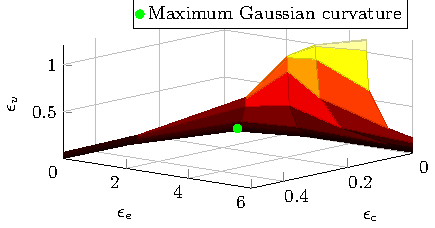
\includegraphics[scale=0.8]{Plots/L3}
\caption{Exemplary parametric surface of the output noise power $\epsilon_v$ versus the dereverberation error energy $\epsilon_c$ and the distortion energy $\epsilon_w$ for the RP-DNR technique.}
\label{fig: L3}
\end{figure}
Although the Gaussian curvature of a surface can be analytically computed, numerical inaccuracies due to the manipulation of large-dimensional matrices can occur when maximizing it~\cite{Belge_IP_2002}, such that a numerically stable algorithm is required.
In this paper, the minimum distance method proposed in~\cite{Belge_IP_2002} has been used to compute the point of maximum Gaussian curvature. 

\section{Simulations}

In this section the dereverberation and noise reduction performance when using the P-MINT filter in~(\ref{eq: w_pmint}), the automatically regularized RP-MINT filter in~(\ref{eq: w_rpmint}), and the automatically parametrized RP-DNR filter in~(\ref{eq: w_rpdnr}) will be evaluated.
% In Section~\ref{sec: expa} the considered acoustic system and the used instrumental performance measures are introduced. 
% In Section~\ref{sec: expb} the influence of the regularization and weighting parameters on the performance of the RP-DNR technique is investigated.
% In Section~\ref{sec: aem}, the automatically parametrized RP-DNR technique is compared to the PMINT and automatically regularized PMINT techniques.

\subsection{Acoustic system and algorithmic settings}

We have considered an acoustic scenario with a single speech source placed in broadside direction to a linear microphone array with $M=4$ equidistant microphones.
The room reverberation time is $T_{60} \approx 610$~ms~\cite{hadad_IWAENC_2014}, the RIR length is $L_h = 4880$, and the sampling frequency is $f_s = 8$ kHz.
The distance between the microphones is $4$~cm and the distance between the speech source and the microphone array is $2$ m.
The speech components in the microphone signals are generated by convolving clean speech signals from the HINT database~\cite{Nilsson_JASA_1994} with the measured RIRs.
The noise components consist of a directional interference and spatially diffuse noise which is simulated using~\cite{Habets2008}.
The directional interference is located in endfire direction at a distance of $2$~m from the microphones.
The broadband input speech-to-interference-ratio~(SIR) is varied between $-5$~dB and $5$~dB and the broadband input speech-to-diffuse-noise-ratio is set to $10$~dB.
The ``speech plus noise'' signal is $13$~s long and is preceded by a $7$~s long ``noise only'' signal, which is not taken into account during evaluation.
\newline
In order to simulate RIR perturbations, the measured RIRs are perturbed by adding scaled white noise as proposed in~\cite{Zhang_HINDAWI_2008}, such that a desired level of normalized projection misalignment~(NPM), i.e.,
\begin{equation}
{\text{NPM}} = 20 \log_{10} \frac{\| \mathbf{h} - \frac{\mathbf{h}^T\hat{\mathbf{h}}}{\hat{\mathbf{h}}^T\hat{\mathbf{h}}}\hat{\mathbf{h}}\|_2}{\| \mathbf{h} \|_2},
\end{equation}
is generated.
The considered NPM values are
\begin{equation}
\label{eq: npm}
{\text{NPM}} \in \{ -33~{\rm{dB}}, \; -27~{\rm{dB}}, \; -21~{\rm{dB}}, \; -15~{\rm{dB}} \}. 
\end{equation}
For all considered techniques the filter length is set equal to $L_w = \left\lceil{\frac{L_h-1}{M-1}}\right\rceil =  1627$, the desired window length is set equal to $L_d = 0.01 \times f_s$, and the target EIR $\mathbf{c}_t$ is chosen as the direct path and early reflections of the perturbed first RIR $\hat{\mathbf{h}}_1$.
In order to generate the L-curve and the L-hypersurface required for the automatic selection of the regularization and weighting parameters, the considered regularization and weighting parameters are
\begin{equation}
\delta, \mu \in \{ 10^{-6}, \; 10^{-5}, \; \ldots, \; 10^{-1}, \; 1, \; 3, \; 5, \; 7 \}.
\end{equation}
Furthermore, the noise correlation matrix is estimated during the ``noise only'' period as
\begin{equation}
\label{eq: corrdiff}
\mathbf{R}_{\mathbf{v}} = \frac{1}{L_v} \sum_{l = 1}^{L_v} \mathbf{v}^{}_l \mathbf{v}^T_l,
\end{equation}
with $L_v$ denoting the number of available ``noise only'' signal vectors.
To avoid other sources of errors, we have assumed that a perfect voice-activity-detector is used.

\subsection{Instrumental performance measures}

The \emph{dereverberation performance} is evaluated in terms of the reverberant energy suppression and perceptual speech quality improvement. 
As commonly done in the evaluation of acoustic multi-channel equalization techniques, the reverberant energy suppression is evaluated as the improvement in direct-to-reverberant ratio~($\Delta$DRR)~\cite{Naylor_Derev_book} between the EIR $c(n)$ and the input RIR $h_1(n)$, i.e., $\Delta {\text{DRR}} = {\text{oDRR}} - {\text{iDRR}}$, with
\begin{equation}
{\text{oDRR}}= 10 \log_{10} \frac{\sum\limits_{n=0}^{n_d-1} c^2(n)}{\sum\limits_{n=n_d}^{L_c-1} c^2(n)}, 
\end{equation}
\begin{equation}
{\text{iDRR}} = 10 \log_{10} \frac{\sum\limits_{n=0}^{n_d-1} h_1^2(n)}{\sum\limits_{n=n_d}^{L_h-1} h_1^2(n)},
\end{equation}
where the first $n_d$ taps of the EIR and RIR represent the direct-path propagation.
The perceptual speech quality is evaluated using the instrumental quality measure PESQ~\cite{PESQ}, which generates a similarity score between a test signal and a reference signal in the range of $1$ to $4.5$. 
The reference signal employed here is $x_{e,1}(n) = s(n) \ast h_{e,1}(n)$, i.e., the early reverberation speech component in the first microphone. 
The improvement in perceptual speech quality $\Delta$PESQ is computed as the difference between the PESQ score of the output speech component $z_x(n)$ and the PESQ score of the reverberant speech component $x_1(n)$.
\newline
The \emph{noise reduction performance} is evaluated in terms of the noise reduction factor $\eta_{_{\rm NR}}$, i.e., 
\begin{equation}
\eta_{_{\rm NR}} = 10 \log_{10} \frac{{\cal{E}} \{v_1^2(n)\}}{{\cal{E}} \{z_v^2(n)\}},
\end{equation}
with $v_1(n)$ the noise component in the first microphone and $z_v(n)$ the output noise component defined in~(\ref{eq: outcomp}).
\newline
The \emph{joint dereverberation and noise reduction performance} is evaluated in terms of the improvement in signal-to-reverberation-and-noise-ratio~($\Delta$SRNR), i.e., $\Delta$SRNR = oSRNR - iSRNR, with 
\begin{align}
{\text{iSRNR}} &= 10 \log_{10} \frac{{\cal{E}} \{x_{e,1}^2(n)\}}{{\cal{E}} \{x_{r,1}^2(n)\} + {\cal{E}} \{v_1^2(n)\}}, \\
{\text{oSRNR}} &= 10 \log_{10} \frac{{\cal{E}} \{z_{e}^2(n)\}}{{\cal{E}} \{z_{r}^2(n)\} + {\cal{E}} \{z_v^2(n)\}},
\end{align}
where $x_{e,1}(n)$ and $x_{r,1}(n)$ are the early and late reverberation speech components in the first microphone defined in~(\ref{eq: ysp}) and $z_e(n)$ and $z_r(n)$ are the early and late reverberation output speech components defined in~(\ref{eq: er_out}) and~(\ref{eq: rr_out}).

\subsection{Results}
\label{sec: exp}

\begin{table*}[t]
\begin{center}
  \caption{Average performance of the P-MINT technique for several input SIR.}
  \label{tbl: perf_pmint}
  \begin{tabularx}{\linewidth}{Xrrrrr}
    \toprule
     Input SIR [dB] & $-5$ & $-2.5$ & $0$ & $2.5$ & $5$ \\
    \midrule
    $\Delta$DRR [dB] & \multicolumn{5}{c}{$-10.8$} \\
    $\Delta$PESQ & \multicolumn{5}{c}{$-0.4$} \\
    $\eta_{_{\rm NR}}$ [dB] & $-28.8$ & $-28.7$ & $-28.4$ & $-28.3$ & $-28.0$ \\
    $\Delta$SRNR [dB] & $-13.1$ & $-12.7$ & $-12.1$ & $-11.2$ & $-10.1$ \\
    \bottomrule
  \end{tabularx}
\end{center}
\end{table*}
\begin{figure*}[t]
\centering
\subfloat[\label{fig: ddrr}]{%
% This file was created by matlab2tikz v0.4.0.
% Copyright (c) 2008--2013, Nico Schlömer <nico.schloemer@gmail.com>
% All rights reserved.
% 
% The latest updates can be retrieved from
%   http://www.mathworks.com/matlabcentral/fileexchange/22022-matlab2tikz
% where you can also make suggestions and rate matlab2tikz.
% 
% 
% 
\begin{tikzpicture}

\begin{axis}[%
width=0.35\figurewidth,
height=\figureheight,
scale only axis,
xmin=-5.5,
xmax=5.5,
ymin=8.7,
ymax=8.85,
xtick = {-5,-2.5,0,2.5,5},
ytick = {8.7,8.75,8.8,8.85},
xlabel absolute, xlabel style={yshift=0.5em},
ylabel absolute, ylabel style={yshift=-0.7em},
xlabel = {Input SIR [dB]},
ylabel = {$\Delta$DRR [dB]},
xmajorgrids,
ymajorgrids,
]
\addplot [
color=blue,
dashed,
mark=o,
line width = 0.8pt,
mark size = 1.7pt,
mark options={solid},
forget plot
]
table[row sep=crcr]{
-5 8.80112686352667\\
-2.5 8.80112686352667\\
0 8.80112686352667\\
2.5 8.80112686352667\\
5 8.80112686352667\\
};
\addplot [
color=green!50!black,
dashed,
mark=square,
line width = 0.8pt,
mark size = 1.7pt,
mark options={solid},
forget plot
]
table[row sep=crcr]{
-5 8.74959626203335\\
-2.5 8.74394033378855\\
0 8.76109777630608\\
2.5 8.77701536289213\\
5 8.79480692234148\\
};
\end{axis}
\end{tikzpicture}%
}
\subfloat[\label{fig: dpesq}]{%
% This file was created by matlab2tikz v0.4.0.
% Copyright (c) 2008--2013, Nico Schlömer <nico.schloemer@gmail.com>
% All rights reserved.
% 
% The latest updates can be retrieved from
%   http://www.mathworks.com/matlabcentral/fileexchange/22022-matlab2tikz
% where you can also make suggestions and rate matlab2tikz.
% 
% 
% 
\begin{tikzpicture}

\begin{axis}[%
width=0.35\figurewidth,
height=\figureheight,
scale only axis,
xmin=-5.5,
xmax=5.5,
ymin=0.59,
ymax=0.62,
xtick = {-5,-2.5,0,2.5,5},
ytick = {0.59,0.6,0.61,0.62},
xlabel absolute, xlabel style={yshift=0.5em},
ylabel absolute, ylabel style={yshift=-0.7em},
xlabel = {Input SIR [dB]},
ylabel = {$\Delta$PESQ},
ymajorgrids,
xmajorgrids,
]
\addplot [
color=blue,
dashed,
mark=o,
line width = 0.8,
mark size = 1.7,
mark options={solid},
forget plot
]
table[row sep=crcr]{
-5 0.6125\\
-2.5 0.6125\\
0 0.6125\\
2.5 0.6125\\
5 0.6125\\
};
\addplot [
color=green!50!black,
dashed,
mark=square,
line width = 0.8,
mark size = 1.7,
mark options={solid},
forget plot
]
table[row sep=crcr]{
-5 0.5965\\
-2.5 0.59475\\
0 0.60275\\
2.5 0.60925\\
5 0.615\\
};
\end{axis}
\end{tikzpicture}%
}
\subfloat[\label{fig: nr}]{%
\hspace{-1.5cm}% This file was created by matlab2tikz v0.4.0.
% Copyright (c) 2008--2013, Nico Schlömer <nico.schloemer@gmail.com>
% All rights reserved.
% 
% The latest updates can be retrieved from
%   http://www.mathworks.com/matlabcentral/fileexchange/22022-matlab2tikz
% where you can also make suggestions and rate matlab2tikz.
% 
% 
% 
\begin{tikzpicture}

\begin{axis}[%
name = nr,
width=0.35\figurewidth,
height=\figureheight,
scale only axis,
xmin=-5.5,
xmax=5.5,
ymin=0.5,
ymax = 6,
xtick = {-5,-2.5,0,2.5,5},
ytick = {1,2,3,4,5,6},
xlabel absolute, xlabel style={yshift=0.5em},
ylabel absolute, ylabel style={yshift=-1.2em},
xlabel = {Input SIR [dB]},
ylabel = {$\eta_{_{\rm NR}}$ [dB]},
ymajorgrids,
legend columns = 2,
legend style={at=({-0.9,1.32}),anchor=north west,row sep = -1.0pt,legend cell align=left,inner sep=0.2pt, outer sep=-0.2pt},
legend entries={{RP-MINT},
                {RP-DNR},
                },
xmajorgrids,
]
\addplot [
color=blue,
dashed,
mark=o,
mark size = 1.7pt,
line width = 0.8pt,
mark options={solid},
]
table[row sep=crcr]{
-5 1.64908912500642\\
-2.5 1.6301508190929\\
0 1.59839640061515\\
2.5 1.54779807445314\\
5 1.47317777054643\\
};
\addplot [
color=green!50!black,
dashed,
mark size = 1.7pt,
line width = 0.8pt,
mark=square,
mark options={solid},
]
table[row sep=crcr]{
-5 5.3446708300213\\
-2.5 5.30523440872317\\
0 4.42192896578351\\
2.5 3.51235048432049\\
5 2.46197284439052\\
};
addlegendentry{RPMINT};
\end{axis}
\end{tikzpicture}%
}
\subfloat[\label{fig: dsrnr}]{%
% This file was created by matlab2tikz v0.4.0.
% Copyright (c) 2008--2013, Nico Schlömer <nico.schloemer@gmail.com>
% All rights reserved.
% 
% The latest updates can be retrieved from
%   http://www.mathworks.com/matlabcentral/fileexchange/22022-matlab2tikz
% where you can also make suggestions and rate matlab2tikz.
% 
% 
% 
\begin{tikzpicture}

\begin{axis}[%
width=0.35\figurewidth,
height=\figureheight,
scale only axis,
xmin=-5.5,
xmax=5.5,
ymin=1.5,
ymax=5,
xtick = {-5,-2.5,0,2.5,5},
ytick = {2,3,4,5},
xlabel absolute, xlabel style={yshift=0.5em},
ylabel absolute, ylabel style={yshift=-1.2em},
xlabel = {Input SIR [dB]},
ylabel = {$\Delta$SRNR [dB]},
ymajorgrids,
xmajorgrids,
]
\addplot [
color=blue,
dashed,
mark=o,
mark size = 1.7pt,
line width = 0.8pt,
mark options={solid},
forget plot
]
table[row sep=crcr]{
-5 2.0464746180046\\
-2.5 2.08197384914999\\
0 2.13014817984129\\
2.5 2.18748815391428\\
5 2.24590987185389\\
};
\addplot [
color=green!50!black,
dashed,
mark=square,
mark size = 1.7pt,
line width = 0.8pt,
mark options={solid},
forget plot
]
table[row sep=crcr]{
-5 4.7946076058636\\
-2.5 4.52578721173842\\
0 3.77323612490486\\
2.5 3.17014502217622\\
5 2.65884152229035\\
};
\end{axis}
\end{tikzpicture}%
}
\caption{Average performance of the automatically regularized P-MINT and the automatically parametrized RP-DNR techniques for several input SIR in terms of (a) $\Delta$DRR, (b) $\Delta$PESQ, (c) $\eta_{_{\rm NR}}$, and (d) $\Delta$SRNR.}
\label{fig: perf_all}
\end{figure*}
\textit{Performance of the P-MINT technique}

To illustrate that the P-MINT technique generally fails to achieve dereverberation and results in additive noise amplification, in this section we only investigate the performance of the P-MINT technique.
The presented performance measures are averaged over the different considered NPM values in~(\ref{eq: npm}).
Table~\ref{tbl: perf_pmint} presents the $\Delta$DRR, $\Delta$PESQ, $\eta_{_{\rm NR}}$, and $\Delta$SRNR values obtained using the P-MINT technique for the different considered input SIRs.
Since the P-MINT reshaping filter is independent of the input SIR, the obtained $\Delta$DRR and $\Delta$PESQ values are the same for all considered input SIRs.
As illustrated, the P-MINT technique fails to achieve dereverberation, worsening the DRR and the PESQ score by $10.8$ dB and $0.4$ respectively.
Furthermore, the noise reduction factors presented in Table~\ref{tbl: perf_pmint} shows that the additive noise is significantly amplified, which is to be expected since the P-MINT reshaping filter is designed without taking the noise statistics into account.
Since the P-MINT technique fails to achieve dereverberation and amplifies the additive noise, it results in a significantly worse SRNR value than in the input signal, as illustrated by the large negative $\Delta$SRNR values presented in Table~\ref{tbl: perf_pmint}.
These simulation results confirm that when the RIR perturbations are not taken into account, acoustic multi-channel equalization techniques fail to achieve dereverberation.
Furthermore, they confirm that designing reshaping filters for speech dereverberation without taking the presence of the additive noise into account results in a large noise amplification.

\textit{Performance of the RP-MINT and RP-DNR techniques}

In this section the performance of the automatically regularized and parametrized RP-MINT and RP-DNR techniques is investigated.
Similarly as before, the presented performance measures are averaged over the different considered NPM values in~(\ref{eq: npm}).
Fig.~\ref{fig: perf_all} depicts the performance of considered techniques in terms of the $\Delta$DRR, $\Delta$PESQ, $\eta_{_{\rm NR}}$, and $\Delta$SRNR measures.
It can be observed in Fig.~\ref{fig: ddrr} that the $\Delta$DRR obtained using the RP-MINT and RP-DNR techniques is very similar, with an insignificant difference of at most $0.05$~dB for low input SIRs.
Furthermore, Fig.~\ref{fig: dpesq} shows that also the PESQ score obtained using the RP-MINT and RP-DNR techniques is very similar, with an insignificant difference of at most $0.02$ for low input SIRs.
These results show that the dereverberation performance of the proposed RP-DNR technique is very similar to the dereverberation performance of the RP-MINT technique.
Although one would expect the dereverberation performance of the RP-DNR technique to be lower than that of the RP-MINT technique, this is not the case in these simulation results.
This occurs due to the automatic selection of the regularization parameter in the RP-MINT technique, which does not yield the best dereverberation performance one would otherwise obtain by intrusively selecting the regularization parameter.
While the dereverberation performance of both techniques is very similar, it can be observed in Fig.~\ref{fig: nr} that the noise reduction factor obtained using the RP-DNR technique is up to $4$~dB higher than the noise reduction factor obtained using the RP-MINT technique.
Furthermore, Fig.~\ref{fig: nr} also shows that the incorporation of regularization in acoustic multi-channel equalization techniques avoids the significantly large noise amplification one would otherwise obtain~(cf. Table~\ref{tbl: perf_pmint}).
This occurs due to the decrease in the reshaping filter energy when regularization is incorporated, which is also partly effective in reducing the distortions in the output signal arising due to the additive noise.
However, it should be noted that there is no guarantee that any noise reduction can be achieved using the RP-MINT technique, since the actual noise statistics are not explicitly taken into account.
The very similar dereverberation performance but higher noise reduction performance of the RP-DNR technique in comparison to the RP-MINT technique is also reflected in the $\Delta$SRNR values depicted in Fig.~\ref{fig: dsrnr}, with the RP-DNR technique yielding a higher $\Delta$SRNR of up to $3$~dB when compared to the RP-MINT technique.
\newline
In summary, these simulation results demonstrate the importance of taking the noise statistics into account in order to achieve joint dereverberation and noise reduction.
Furthermore they show that the proposed RP-DNR technique does not sacrifice the high dereverberation performance of the RP-MINT technique, but improves the noise reduction as well as the joint dereverberation and noise reduction performance.


\section{Conclusion}

In this paper we have proposed the RP-DNR technique which aims at joint dereverberation and noise reduction based on acoustic multi-channel equalization.
The RP-DNR technique directly extends the RP-MINT technique by explicitly taking the noise statistics into account. 
In addition to the regularization parameter used in the RP-MINT technique, the RP-DNR technique introduces an additional weighting parameter, enabling to trade off between dereverberation and noise reduction.
We have also proposed an automatic non-intrusive procedure based on the L-hypersurface for selecting the regularization and weighting parameters.
Simulation results demonstrate that the RP-DNR technique maintains the high dereverberation performance of the RP-MINT technique, while improving the noise reduction as well as the joint dereverberation and noise reduction performance.

\small
\bibliographystyle{IEEEtran}
\bibliography{refs}
% \begin{thebibliography}{99}



% \bibitem{DEK1}
% Author, ``Title,'' presented at the AES 114th convention, 
% Amsterdam, The Netherlands, 2003 March 22--25. 

% %\bibitem{DEK2}
% %D. E. Knuth, {\it Selected papers on analysis of algorithms}, CSLI
% %Publ., Stanford, CA, 2000; CNO
% %CMP 1 762 319 
% %
% %\bibitem{DEK3}
% %D. E. Knuth, Algorithmica {\bf 22} (1998), no.~4, 561--568; MR
% %2000j:68037 
% %
% %\bibitem{DEK4}
% %R. L. Graham, D. E. Knuth and O. Patashnik, {\it Concrete mathematics}
% %(Polish), Translated from the
% %second English (1994) edition by P. Chrzastowski, A. Czumaj,
% %L. Gasieniec and M. Raczunas, Second
% %edition, Wydawnictwo Naukowe PWN, Warsaw, 1998; MR 99m:68002
% %
% \end{thebibliography}


\end{document}